\documentclass[12pt,a4paper]{article}
\usepackage[margin=0.9in]{geometry}
\usepackage{graphicx}
\usepackage{booktabs}
\usepackage{hyperref}
\usepackage{float}
\usepackage{subcaption}
\usepackage{amsmath}
\usepackage{xcolor}

\title{\textbf{Assignment 5 --- MLOps} \\ ViT Fine-tuning with LoRA \& Adversarial Attacks}
\author{Tejas Gupta \\ B22CS093 \\ IIT Jodhpur}
\date{}

\begin{document}
\maketitle

\section*{Links}
\begin{itemize}
    \item \textbf{GitHub:} \url{https://github.com/TejasGupta-27/MLOps-TejasGupta-B22CS093/tree/Assignment5}
    \item \textbf{WandB (Q1):} \url{https://wandb.ai/b22cs093-prom-iit-rajasthan/vit-lora-cifar100}
    \item \textbf{WandB (Q2):} \url{https://wandb.ai/b22cs093-prom-iit-rajasthan/adversarial-cifar10}
    \item \textbf{HuggingFace:} \url{https://huggingface.co/Tron2703/vit-lora-cifar100}
\end{itemize}

All experiments were run inside a Docker container on an NVIDIA RTX A5000 (24\,GB) GPU using PyTorch with mixed-precision (FP16) training.

%======================================================================
\section{Q1: ViT-S Fine-tuning with LoRA on CIFAR-100}
%======================================================================

\subsection{Setup}
\begin{itemize}
    \item \textbf{Model:} \texttt{vit\_small\_patch16\_224} (timm), pre-trained on ImageNet-1K.
    \item \textbf{Dataset:} CIFAR-100 resized to $224\times224$, 90/10 train-val split.
    \item \textbf{LoRA:} Injected into Q, K, V attention weights via the PEFT library.
    \item \textbf{Training:} 10 epochs, AdamW (lr\,$=10^{-3}$), cosine annealing, batch size 128.
    \item \textbf{Dropout:} 0.1 for all LoRA experiments.
\end{itemize}

%----------------------------------------------------------------------
\subsection{Experiment 1 (No LoRA): Head-only Fine-tuning}
Trainable Parameters: \textbf{38,500} (classification head only).

\begin{table}[H]
\centering
\caption{Experiment 1 --- No LoRA}
\small
\begin{tabular}{ccccc}
\toprule
Epoch & Train Loss & Val Loss & Train Acc (\%) & Val Acc (\%) \\
\midrule
1  & 1.0235 & 0.7360 & 73.82 & 79.54 \\
2  & 0.5860 & 0.6770 & 82.76 & 80.72 \\
3  & 0.5149 & 0.6661 & 84.46 & 80.68 \\
4  & 0.4668 & 0.6640 & 85.66 & 81.08 \\
5  & 0.4353 & 0.6552 & 86.70 & 81.12 \\
6  & 0.4025 & 0.6525 & 87.65 & 81.24 \\
7  & 0.3832 & 0.6436 & 88.13 & 81.68 \\
8  & 0.3649 & 0.6415 & 88.84 & 81.58 \\
9  & 0.3508 & 0.6375 & 89.36 & 81.38 \\
10 & 0.3439 & 0.6379 & 89.51 & 81.40 \\
\bottomrule
\end{tabular}
\end{table}

%----------------------------------------------------------------------
\subsection{Experiment 2: Rank=2, Alpha=2}
Trainable Parameters: \textbf{36,864}.

\begin{table}[H]
\centering
\caption{Experiment 2 --- LoRA R=2, $\alpha$=2, Dropout=0.1}
\small
\begin{tabular}{ccccc}
\toprule
Epoch & Train Loss & Val Loss & Train Acc (\%) & Val Acc (\%) \\
\midrule
1  & 3.3436 & 2.3649 & 24.61 & 44.26 \\
2  & 2.0346 & 1.8988 & 54.03 & 58.12 \\
3  & 1.7212 & 1.7152 & 62.38 & 62.14 \\
4  & 1.5637 & 1.6098 & 66.47 & 64.46 \\
5  & 1.4661 & 1.5434 & 68.56 & 66.14 \\
6  & 1.3970 & 1.4898 & 70.41 & 67.20 \\
7  & 1.3501 & 1.4600 & 71.54 & 67.20 \\
8  & 1.3164 & 1.4361 & 72.50 & 68.60 \\
9  & 1.2928 & 1.4330 & 73.14 & 68.44 \\
10 & 1.2820 & 1.4262 & 73.24 & 68.60 \\
\bottomrule
\end{tabular}
\end{table}

%----------------------------------------------------------------------
\subsection{Experiment 3: Rank=2, Alpha=4}
Trainable Parameters: \textbf{36,864}.

\begin{table}[H]
\centering
\caption{Experiment 3 --- LoRA R=2, $\alpha$=4, Dropout=0.1}
\small
\begin{tabular}{ccccc}
\toprule
Epoch & Train Loss & Val Loss & Train Acc (\%) & Val Acc (\%) \\
\midrule
1  & 3.0484 & 2.2490 & 32.78 & 51.02 \\
2  & 1.8777 & 1.8658 & 59.44 & 60.22 \\
3  & 1.6193 & 1.6975 & 65.23 & 64.00 \\
4  & 1.4826 & 1.5806 & 68.56 & 66.54 \\
5  & 1.3953 & 1.5206 & 70.70 & 68.02 \\
6  & 1.3238 & 1.4590 & 72.45 & 69.82 \\
7  & 1.2781 & 1.4350 & 73.72 & 70.24 \\
8  & 1.2400 & 1.4100 & 74.41 & 70.54 \\
9  & 1.2160 & 1.3966 & 75.04 & 70.60 \\
10 & 1.2032 & 1.3923 & 75.56 & 70.86 \\
\bottomrule
\end{tabular}
\end{table}

%----------------------------------------------------------------------
\subsection{Experiment 4: Rank=2, Alpha=8}
Trainable Parameters: \textbf{36,864}.

\begin{table}[H]
\centering
\caption{Experiment 4 --- LoRA R=2, $\alpha$=8, Dropout=0.1}
\small
\begin{tabular}{ccccc}
\toprule
Epoch & Train Loss & Val Loss & Train Acc (\%) & Val Acc (\%) \\
\midrule
1  & 2.9794 & 2.0348 & 32.27 & 54.46 \\
2  & 1.8107 & 1.6815 & 59.51 & 62.68 \\
3  & 1.5556 & 1.5441 & 65.93 & 66.14 \\
4  & 1.4142 & 1.4437 & 69.56 & 68.12 \\
5  & 1.3280 & 1.3610 & 72.00 & 70.36 \\
6  & 1.2637 & 1.3236 & 73.63 & 71.36 \\
7  & 1.2106 & 1.2973 & 75.05 & 71.68 \\
8  & 1.1703 & 1.2659 & 76.14 & 72.76 \\
9  & 1.1426 & 1.2556 & 76.91 & 73.10 \\
10 & 1.1268 & 1.2400 & 77.18 & 73.06 \\
\bottomrule
\end{tabular}
\end{table}

%----------------------------------------------------------------------
\subsection{Experiment 5: Rank=4, Alpha=2}
Trainable Parameters: \textbf{73,728}.

\begin{table}[H]
\centering
\caption{Experiment 5 --- LoRA R=4, $\alpha$=2, Dropout=0.1}
\small
\begin{tabular}{ccccc}
\toprule
Epoch & Train Loss & Val Loss & Train Acc (\%) & Val Acc (\%) \\
\midrule
1  & 3.3300 & 2.3193 & 24.78 & 44.68 \\
2  & 1.8309 & 1.7354 & 57.22 & 59.68 \\
3  & 1.4614 & 1.5082 & 67.11 & 66.12 \\
4  & 1.2622 & 1.3512 & 71.93 & 68.94 \\
5  & 1.1424 & 1.2695 & 74.80 & 72.14 \\
6  & 1.0592 & 1.2207 & 76.72 & 72.80 \\
7  & 1.0024 & 1.1756 & 78.21 & 73.64 \\
8  & 0.9635 & 1.1571 & 79.18 & 74.38 \\
9  & 0.9378 & 1.1415 & 79.80 & 74.56 \\
10 & 0.9253 & 1.1408 & 80.21 & 74.70 \\
\bottomrule
\end{tabular}
\end{table}

%----------------------------------------------------------------------
\subsection{Experiment 6: Rank=4, Alpha=4}
Trainable Parameters: \textbf{73,728}.

\begin{table}[H]
\centering
\caption{Experiment 6 --- LoRA R=4, $\alpha$=4, Dropout=0.1}
\small
\begin{tabular}{ccccc}
\toprule
Epoch & Train Loss & Val Loss & Train Acc (\%) & Val Acc (\%) \\
\midrule
1  & 2.9392 & 1.8776 & 33.82 & 56.52 \\
2  & 1.5459 & 1.3755 & 65.70 & 70.18 \\
3  & 1.2223 & 1.1668 & 73.58 & 74.98 \\
4  & 1.0521 & 1.0632 & 77.67 & 77.52 \\
5  & 0.9503 & 0.9848 & 79.77 & 79.06 \\
6  & 0.8804 & 0.9370 & 81.56 & 80.24 \\
7  & 0.8288 & 0.9092 & 82.92 & 80.62 \\
8  & 0.7908 & 0.8898 & 83.87 & 80.58 \\
9  & 0.7689 & 0.8802 & 84.26 & 80.88 \\
10 & 0.7575 & 0.8721 & 84.60 & 81.24 \\
\bottomrule
\end{tabular}
\end{table}

%----------------------------------------------------------------------
\subsection{Experiment 7: Rank=4, Alpha=8}
Trainable Parameters: \textbf{73,728}.

\begin{table}[H]
\centering
\caption{Experiment 7 --- LoRA R=4, $\alpha$=8, Dropout=0.1}
\small
\begin{tabular}{ccccc}
\toprule
Epoch & Train Loss & Val Loss & Train Acc (\%) & Val Acc (\%) \\
\midrule
1  & 2.6024 & 1.5670 & 41.99 & 66.30 \\
2  & 1.2907 & 1.1959 & 72.12 & 73.74 \\
3  & 1.0309 & 1.0728 & 77.72 & 75.56 \\
4  & 0.9004 & 0.9566 & 80.67 & 78.76 \\
5  & 0.8125 & 0.9151 & 82.69 & 79.26 \\
6  & 0.7535 & 0.8754 & 83.99 & 79.46 \\
7  & 0.7052 & 0.8534 & 85.37 & 80.58 \\
8  & 0.6671 & 0.8316 & 86.48 & 80.98 \\
9  & 0.6417 & 0.8249 & 87.20 & 80.66 \\
10 & 0.6284 & 0.8192 & 87.41 & 80.88 \\
\bottomrule
\end{tabular}
\end{table}

%----------------------------------------------------------------------
\subsection{Experiment 8: Rank=8, Alpha=2}
Trainable Parameters: \textbf{147,456}.

\begin{table}[H]
\centering
\caption{Experiment 8 --- LoRA R=8, $\alpha$=2, Dropout=0.1}
\small
\begin{tabular}{ccccc}
\toprule
Epoch & Train Loss & Val Loss & Train Acc (\%) & Val Acc (\%) \\
\midrule
1  & 3.3195 & 2.1397 & 26.03 & 51.04 \\
2  & 1.6880 & 1.4772 & 61.24 & 66.08 \\
3  & 1.2464 & 1.1762 & 71.62 & 73.10 \\
4  & 1.0178 & 1.0272 & 76.71 & 76.72 \\
5  & 0.8815 & 0.9349 & 80.04 & 78.60 \\
6  & 0.7917 & 0.8800 & 82.19 & 79.16 \\
7  & 0.7352 & 0.8366 & 83.47 & 80.58 \\
8  & 0.6979 & 0.8149 & 84.40 & 81.20 \\
9  & 0.6745 & 0.8052 & 84.93 & 81.18 \\
10 & 0.6623 & 0.8010 & 85.18 & 81.32 \\
\bottomrule
\end{tabular}
\end{table}

%----------------------------------------------------------------------
\subsection{Experiment 9: Rank=8, Alpha=4}
Trainable Parameters: \textbf{147,456}.

\begin{table}[H]
\centering
\caption{Experiment 9 --- LoRA R=8, $\alpha$=4, Dropout=0.1}
\small
\begin{tabular}{ccccc}
\toprule
Epoch & Train Loss & Val Loss & Train Acc (\%) & Val Acc (\%) \\
\midrule
1  & 2.9010 & 1.7009 & 34.47 & 59.58 \\
2  & 1.3090 & 1.1719 & 69.36 & 72.18 \\
3  & 0.9583 & 0.9683 & 77.68 & 77.30 \\
4  & 0.7908 & 0.8713 & 81.49 & 78.88 \\
5  & 0.6915 & 0.7906 & 83.75 & 81.02 \\
6  & 0.6207 & 0.7684 & 85.61 & 81.50 \\
7  & 0.5718 & 0.7372 & 86.80 & 82.06 \\
8  & 0.5365 & 0.7271 & 87.85 & 82.06 \\
9  & 0.5146 & 0.7156 & 88.42 & 82.24 \\
10 & 0.5045 & 0.7142 & 88.79 & 82.54 \\
\bottomrule
\end{tabular}
\end{table}

%----------------------------------------------------------------------
\subsection{Experiment 10: Rank=8, Alpha=8}
Trainable Parameters: \textbf{147,456}.

\begin{table}[H]
\centering
\caption{Experiment 10 --- LoRA R=8, $\alpha$=8, Dropout=0.1}
\small
\begin{tabular}{ccccc}
\toprule
Epoch & Train Loss & Val Loss & Train Acc (\%) & Val Acc (\%) \\
\midrule
1  & 2.6181 & 1.3861 & 40.24 & 68.44 \\
2  & 1.0836 & 0.9385 & 75.07 & 78.14 \\
3  & 0.7863 & 0.7919 & 81.90 & 81.60 \\
4  & 0.6432 & 0.7200 & 85.15 & 82.64 \\
5  & 0.5538 & 0.6691 & 87.31 & 83.92 \\
6  & 0.4899 & 0.6355 & 89.05 & 84.56 \\
7  & 0.4466 & 0.6161 & 90.22 & 84.88 \\
8  & 0.4138 & 0.6053 & 91.17 & 85.18 \\
9  & 0.3892 & 0.6025 & 91.85 & 85.08 \\
10 & 0.3769 & 0.5999 & 92.41 & 85.22 \\
\bottomrule
\end{tabular}
\end{table}

%----------------------------------------------------------------------
\subsection{Test Results Summary}

\begin{table}[H]
\centering
\caption{Overall Test Accuracy across all configurations}
\begin{tabular}{lccccc}
\toprule
LoRA & Rank & Alpha & Dropout & Test Acc (\%) & Trainable Params \\
\midrule
Without & -- & -- & -- & 81.11 & 38,500 \\
With & 2 & 2 & 0.1 & 68.54 & 36,864 \\
With & 2 & 4 & 0.1 & 70.10 & 36,864 \\
With & 2 & 8 & 0.1 & 72.55 & 36,864 \\
With & 4 & 2 & 0.1 & 74.45 & 73,728 \\
With & 4 & 4 & 0.1 & 80.10 & 73,728 \\
With & 4 & 8 & 0.1 & 80.96 & 73,728 \\
With & 8 & 2 & 0.1 & 81.26 & 147,456 \\
With & 8 & 4 & 0.1 & 82.96 & 147,456 \\
\textbf{With} & \textbf{8} & \textbf{8} & \textbf{0.1} & \textbf{85.40} & \textbf{147,456} \\
\bottomrule
\end{tabular}
\end{table}

%----------------------------------------------------------------------
\subsection{Analysis of Q1 Results}

\textbf{Effect of Rank.}
Increasing the LoRA rank from 2 to 8 consistently improves both validation and test accuracy.
At rank\,=\,2, the LoRA models (36,864 trainable params) \emph{underperform} the head-only baseline (38,500 params), indicating that the low-rank bottleneck is too restrictive for the QKV adaptation required.
At rank\,=\,8, LoRA models (147,456 params) comfortably surpass the baseline.
Higher rank allows the low-rank matrices to span a richer subspace of weight updates, enabling more expressive fine-tuning of the attention mechanism.

\textbf{Effect of Alpha.}
For every fixed rank, raising alpha from 2 to 8 improves performance.
Alpha controls the scaling factor $\alpha / r$ applied to the LoRA update $\Delta W = \frac{\alpha}{r} B A$.
A larger alpha amplifies the learned perturbation, allowing LoRA to make more meaningful adjustments to the frozen attention weights.
The best configuration (R\,=\,8, $\alpha$\,=\,8) achieves \textbf{85.40\%} test accuracy---4.29 percentage points above the head-only baseline.

\textbf{Parameter Efficiency.}
Even the best LoRA model uses only 147,456 trainable parameters, which is 0.68\% of the full 21.7M ViT-S model.
This demonstrates the strong parameter efficiency of LoRA for transfer learning on CIFAR-100.

\textbf{Convergence.}
Low-rank/low-alpha configurations (e.g.\ R\,=\,2, $\alpha$\,=\,2) converge slowly and plateau at lower accuracy, while R\,=\,8, $\alpha$\,=\,8 converges faster and reaches higher final accuracy, suggesting that the scaling factor plays a critical role in training dynamics.

%----------------------------------------------------------------------
\subsection{Class-wise Test Accuracy Histograms}

\begin{figure}[H]
\centering
\begin{subfigure}{0.48\textwidth}
    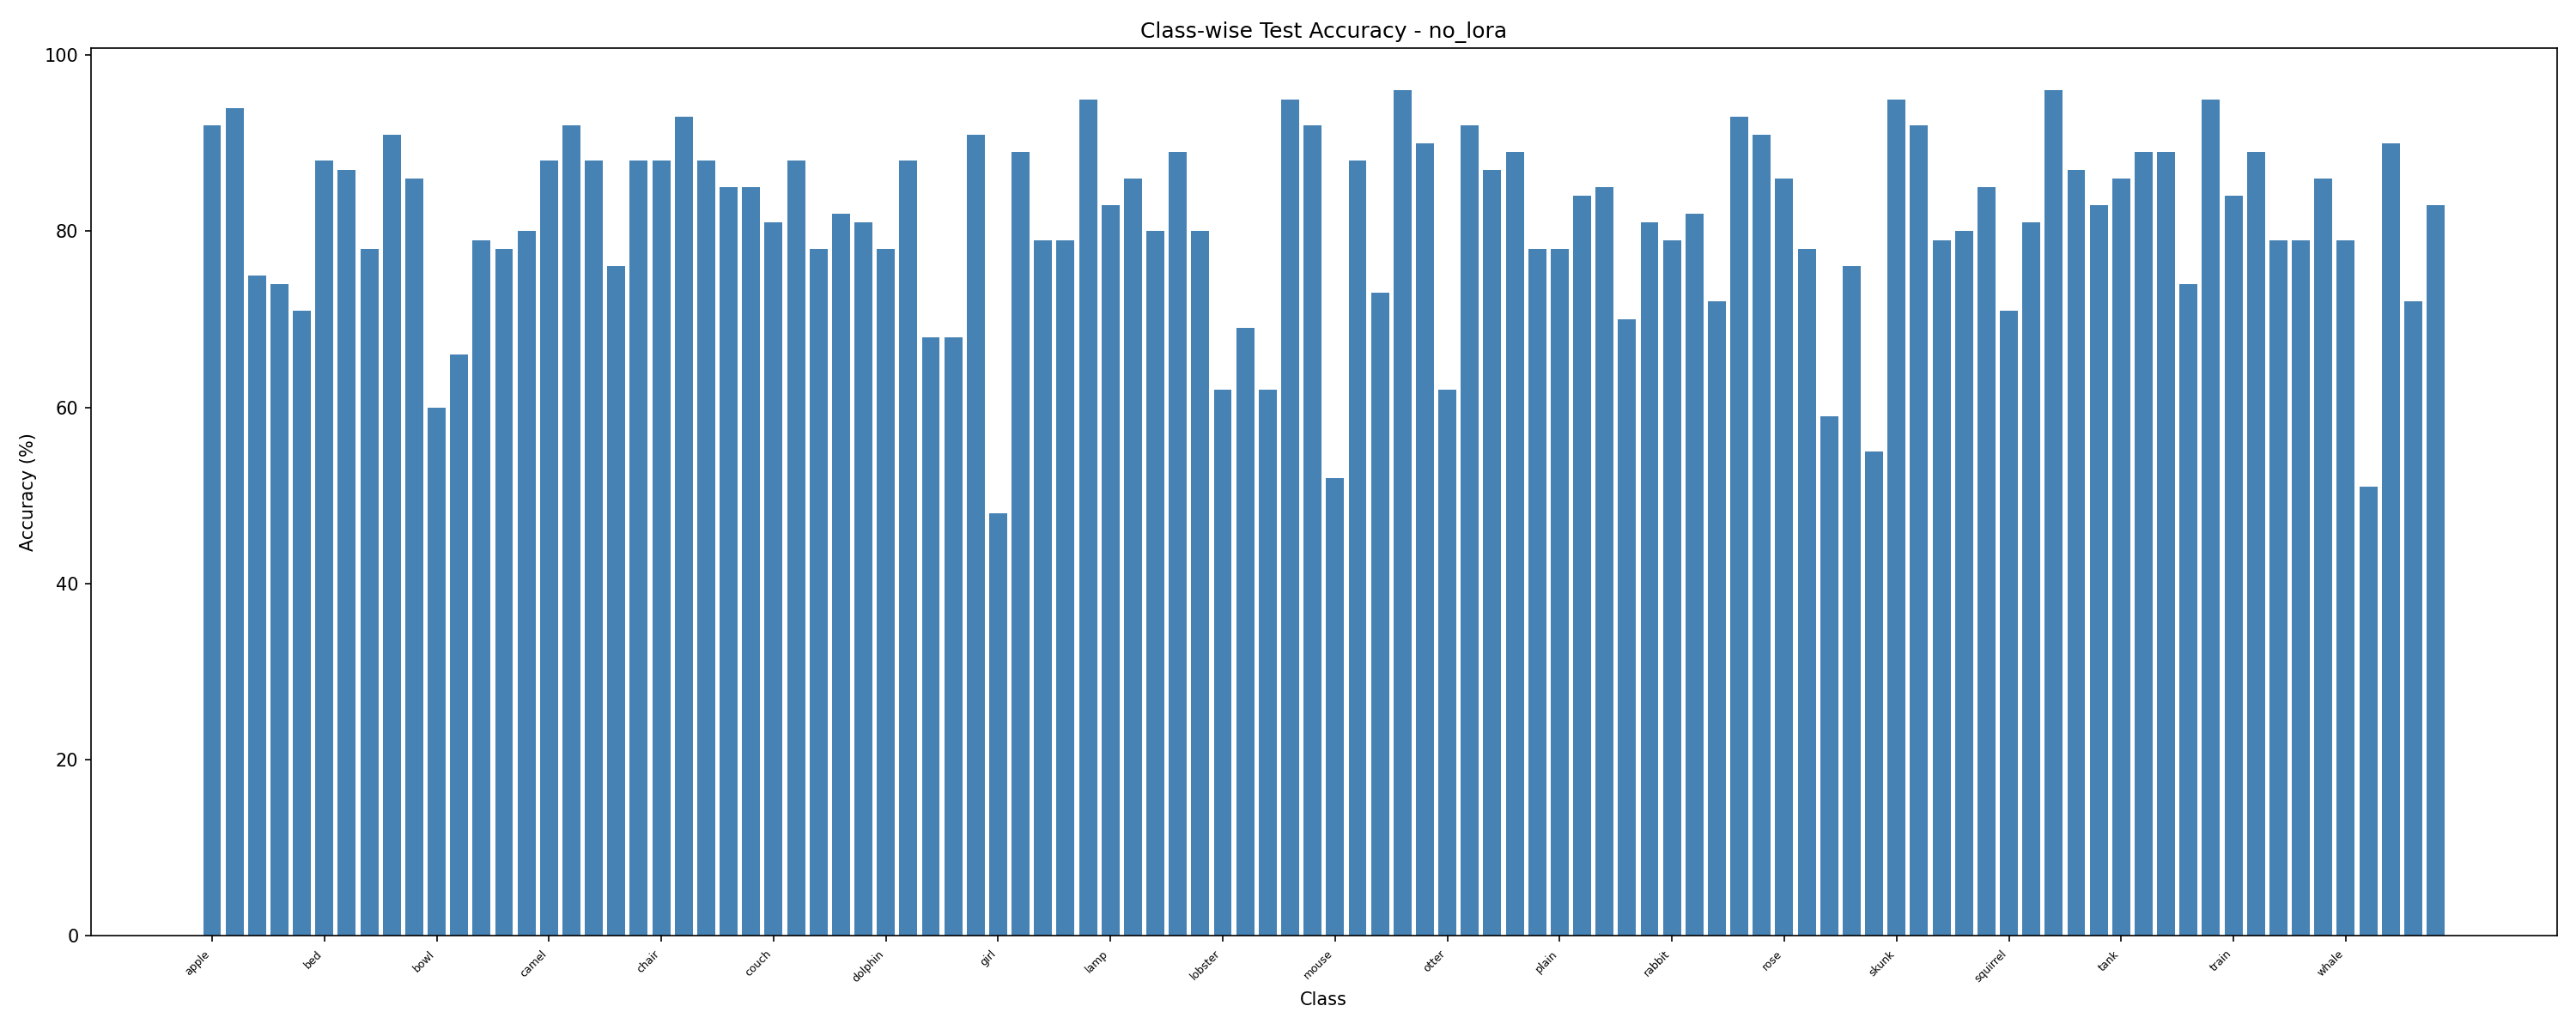
\includegraphics[width=\textwidth]{figures/class_acc_no_lora.png}
    \caption{No LoRA (baseline)}
\end{subfigure}
\begin{subfigure}{0.48\textwidth}
    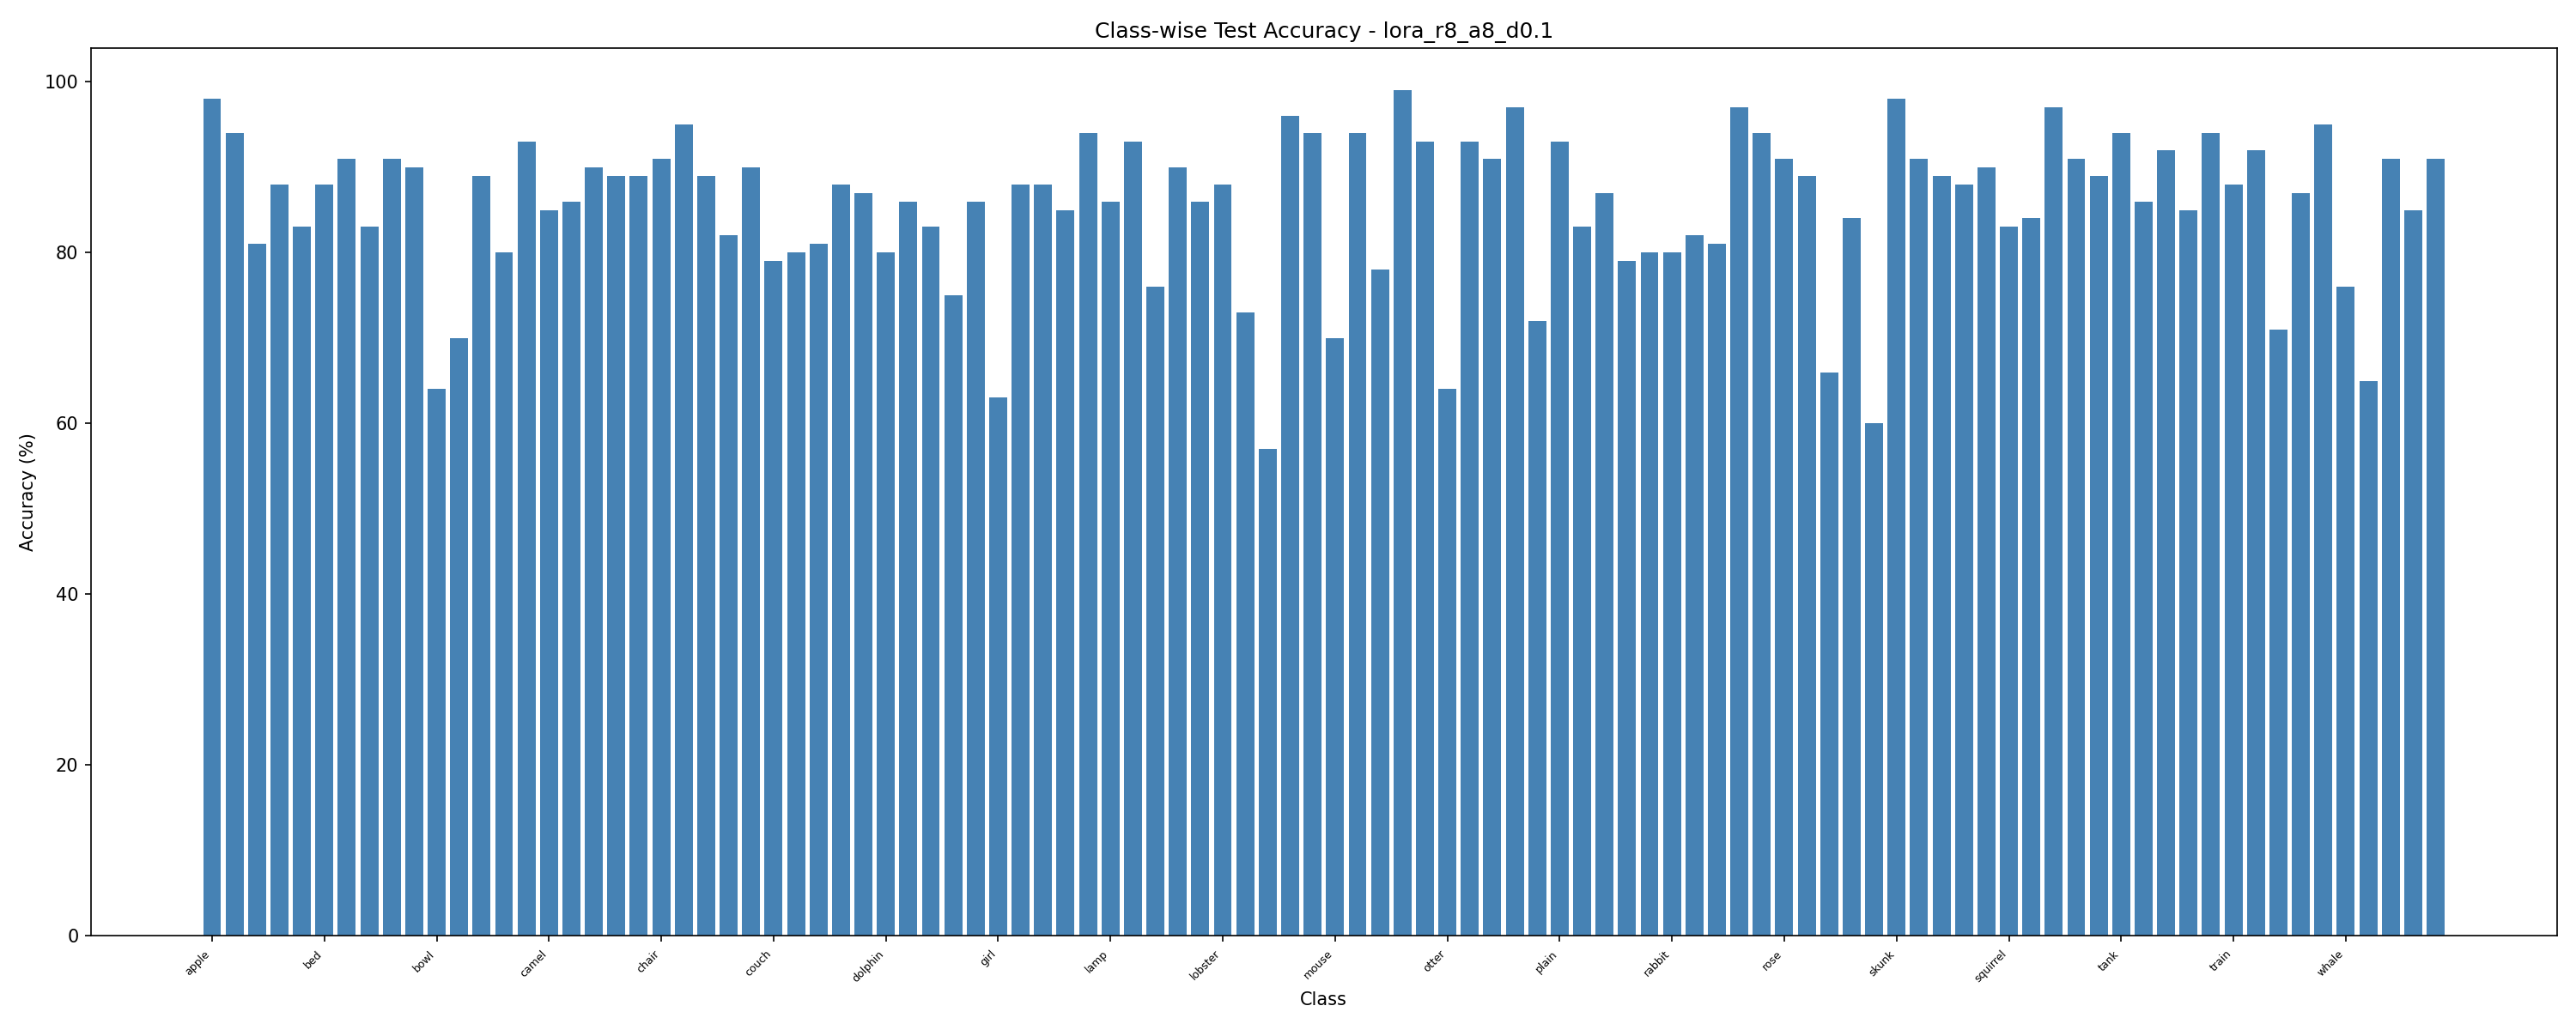
\includegraphics[width=\textwidth]{figures/class_acc_lora_r8_a8_d0.1.png}
    \caption{LoRA R=8, $\alpha$=8 (best)}
\end{subfigure}
\caption{Class-wise test accuracy for the baseline and best LoRA configuration. The LoRA model shows more uniform accuracy across classes.}
\end{figure}

\begin{figure}[H]
\centering
\begin{subfigure}{0.32\textwidth}
    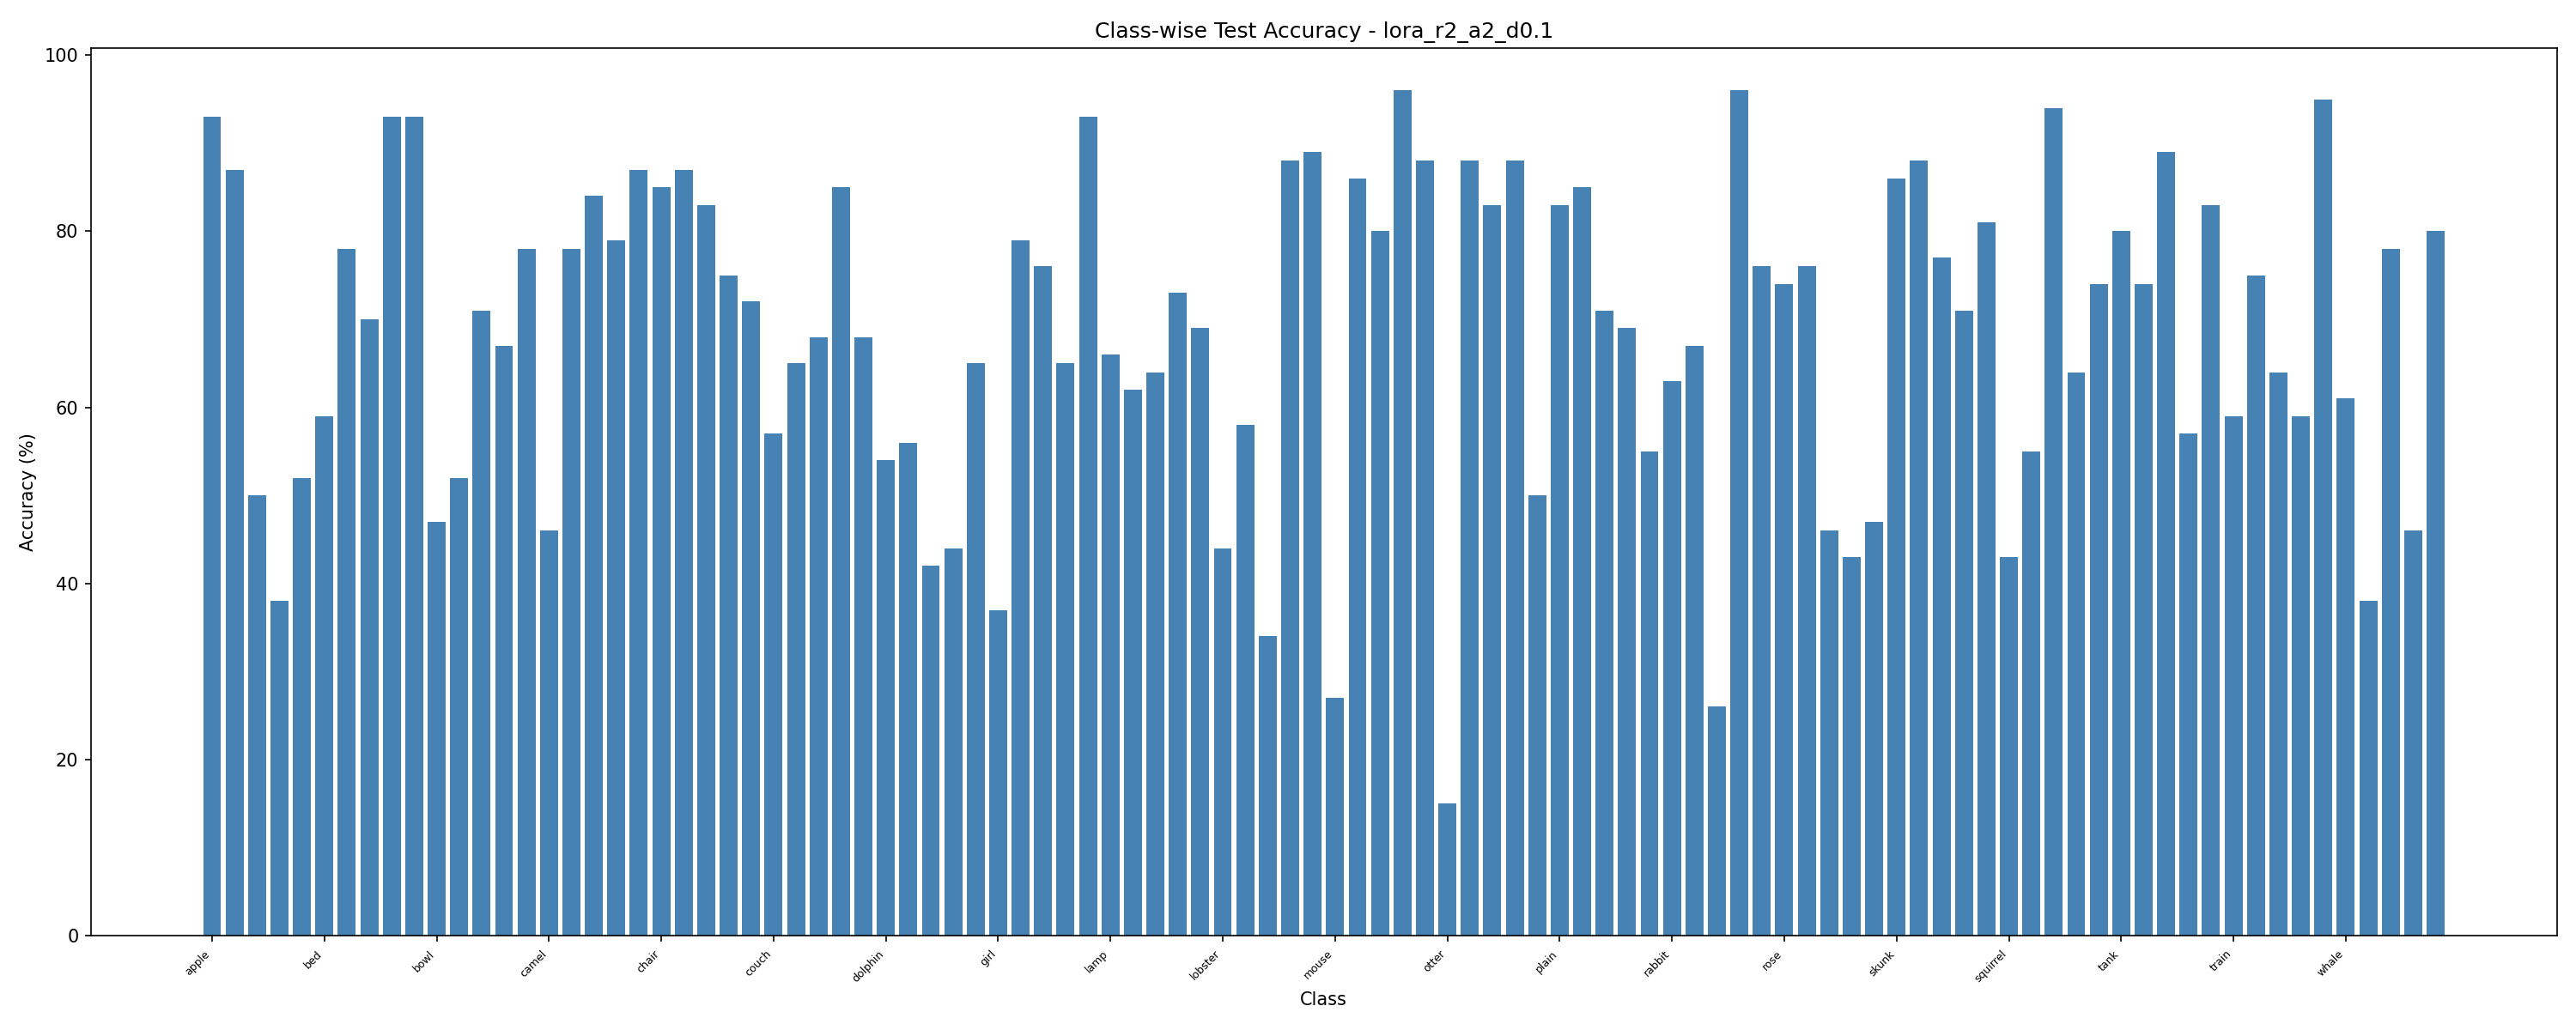
\includegraphics[width=\textwidth]{figures/class_acc_lora_r2_a2_d0.1.png}
    \caption{R=2, $\alpha$=2}
\end{subfigure}
\begin{subfigure}{0.32\textwidth}
    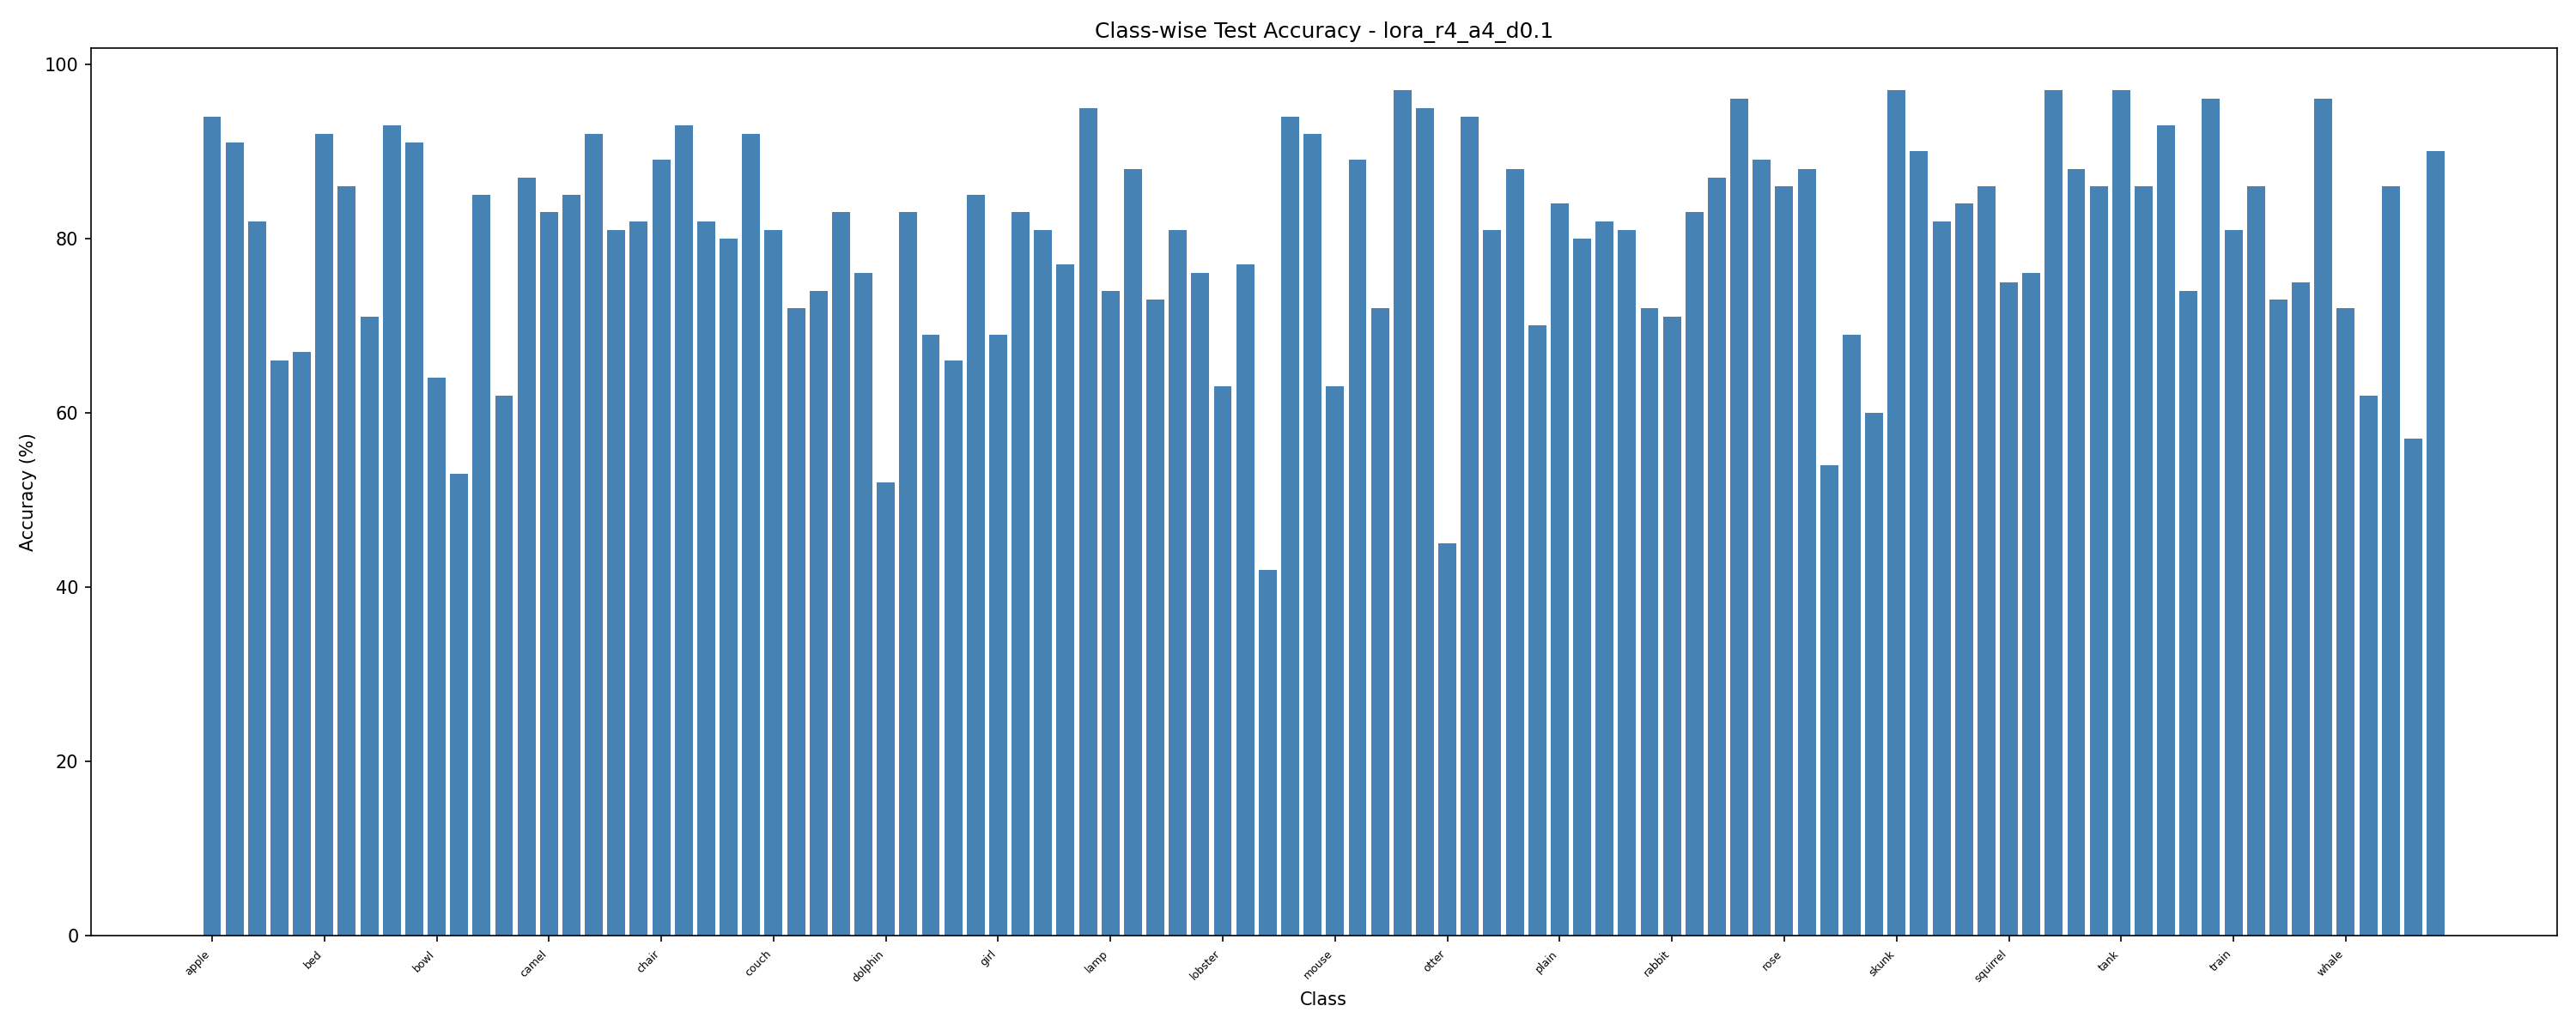
\includegraphics[width=\textwidth]{figures/class_acc_lora_r4_a4_d0.1.png}
    \caption{R=4, $\alpha$=4}
\end{subfigure}
\begin{subfigure}{0.32\textwidth}
    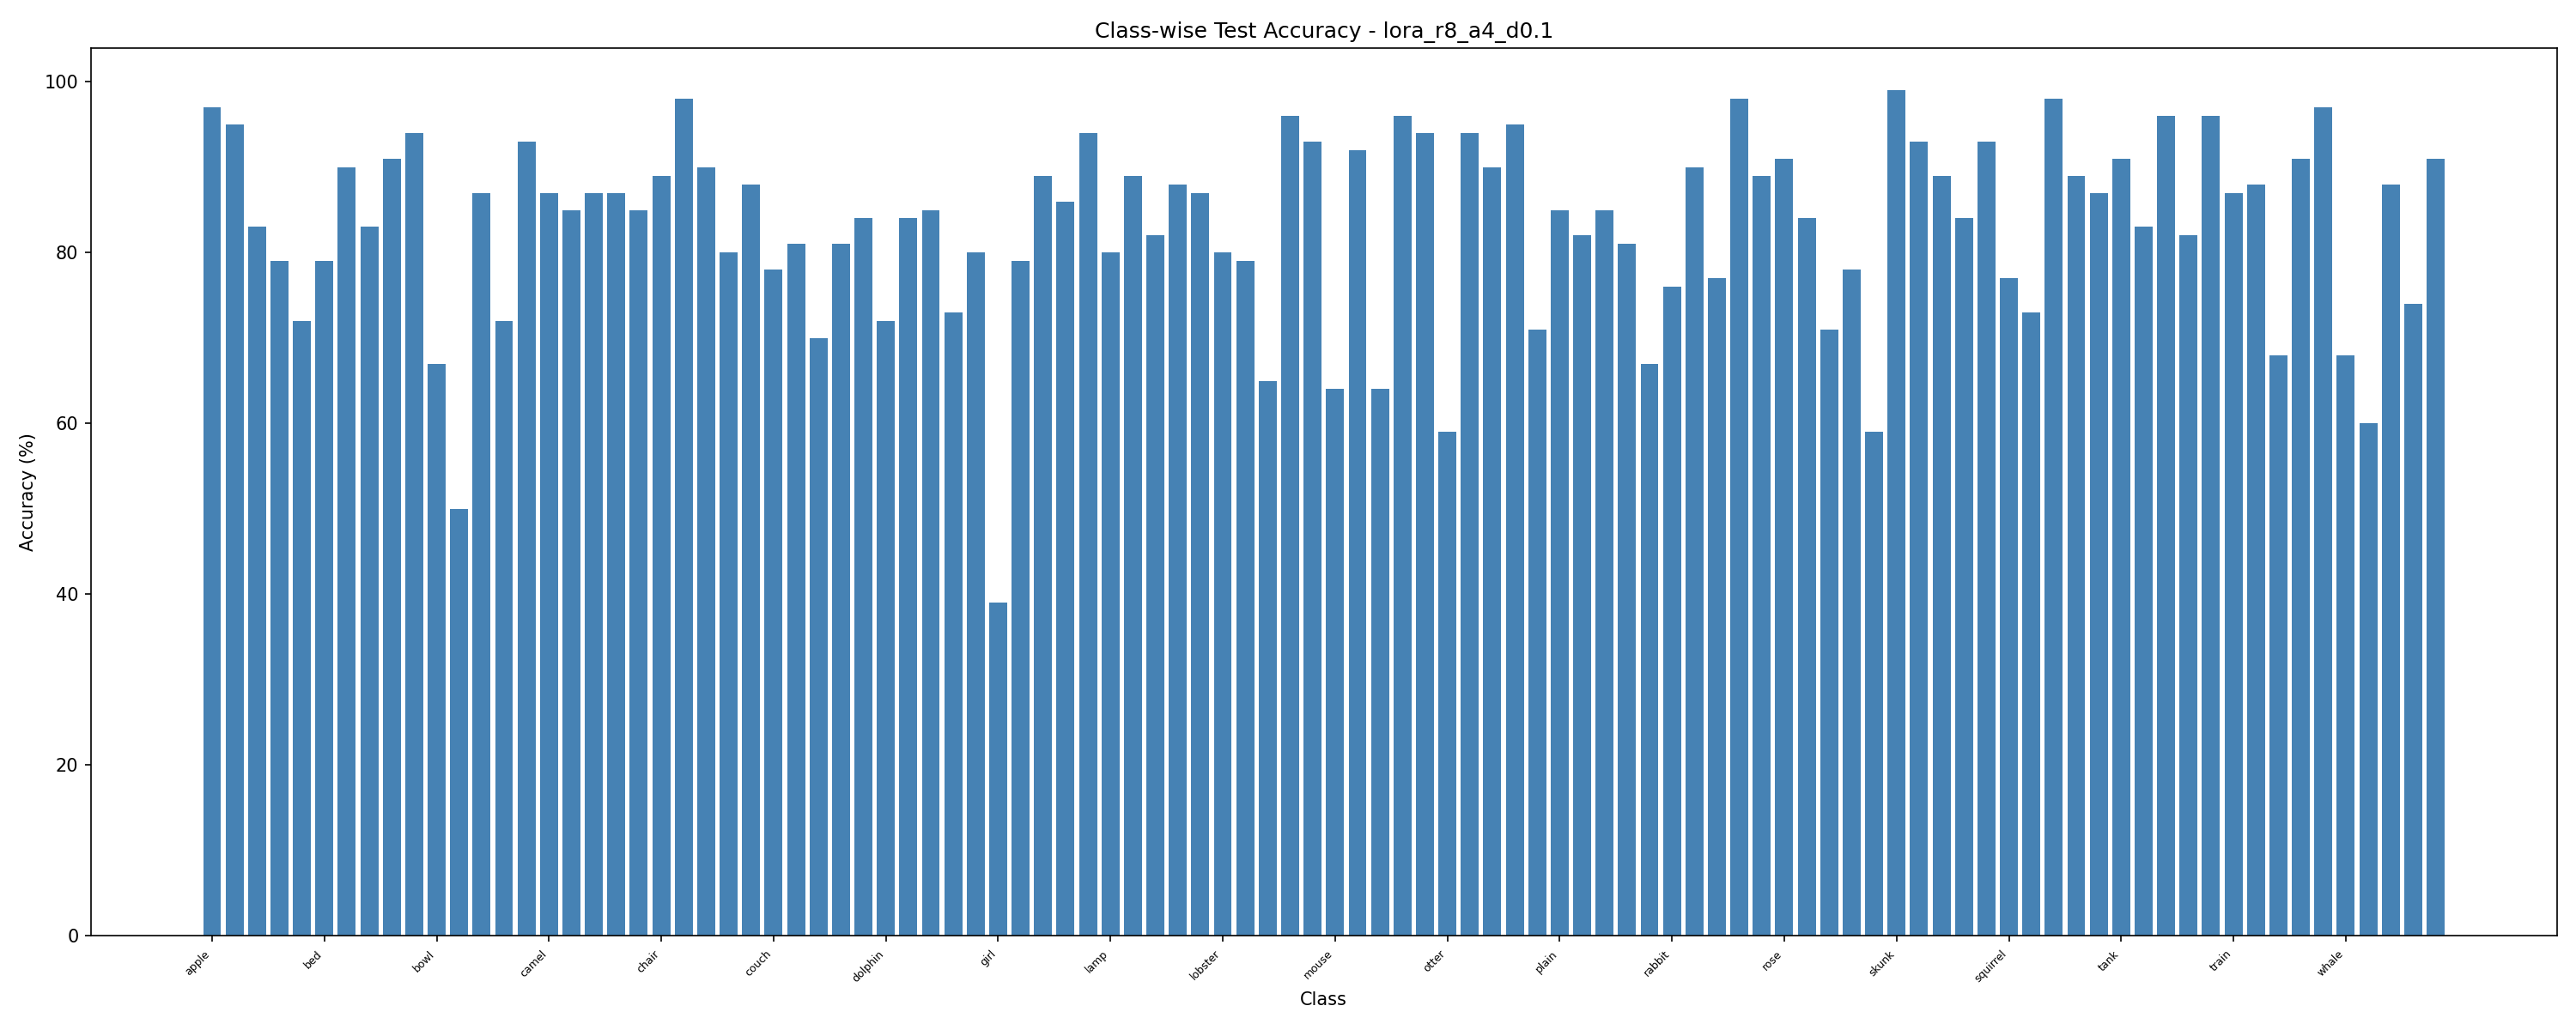
\includegraphics[width=\textwidth]{figures/class_acc_lora_r8_a4_d0.1.png}
    \caption{R=8, $\alpha$=4}
\end{subfigure}
\caption{Class-wise accuracy for selected LoRA configurations, showing progressive improvement with increasing rank and alpha.}
\end{figure}

%----------------------------------------------------------------------
\subsection{Gradient Update Graphs on LoRA Weights}

Gradient norms on LoRA parameters (lora\_A and lora\_B matrices across all attention layers) were logged to WandB at every training step.
The gradients show a clear decreasing trend over training, consistent with the cosine annealing learning rate schedule.
Higher-rank configurations exhibit larger initial gradient magnitudes but converge to similar small values.
The full gradient norm plots are available on the WandB dashboard:
\url{https://wandb.ai/b22cs093-prom-iit-rajasthan/vit-lora-cifar100}

%----------------------------------------------------------------------
\subsection{Optuna Hyperparameter Search}

Optuna was used to search over rank $\in \{2,4,8\}$, alpha $\in \{2,4,8\}$, and learning rate (log-uniform in $[10^{-4}, 10^{-2}]$) with 20 trials and median pruning.

\textbf{Best configuration found:}
\begin{itemize}
    \item Rank = 8, Alpha = 8, LR = 0.00564
    \item Best Validation Accuracy: \textbf{87.56\%}
\end{itemize}

This confirms the grid-search finding that higher rank and alpha are optimal. The Optuna-tuned learning rate (0.00564) is $\sim$5.6$\times$ higher than the default ($10^{-3}$), indicating that LoRA parameters benefit from a more aggressive learning rate since only a small fraction of the network is being updated.

The best Optuna model weights are pushed to GitHub (\texttt{weights/best\_optuna\_model.pth}) and HuggingFace.

%======================================================================
\newpage
\section{Q2: Adversarial Attacks using IBM ART}
%======================================================================

\subsection{Q2(i): FGSM Attack --- From Scratch vs IBM ART}

\subsubsection{ResNet18 Training on CIFAR-10}
A ResNet18 model (modified for CIFAR-10: $3\times3$ first conv, removed maxpool) was trained from scratch for 50 epochs using SGD (lr\,=\,0.1, momentum\,=\,0.9, milestones at epochs 20/35/45).

\textbf{Best Test Accuracy: 93.34\%} (well above the 72\% threshold).

\subsubsection{FGSM Implementation}
\textbf{From Scratch:} Computed the gradient of the cross-entropy loss w.r.t.\ the input image, then perturbed each pixel by $\epsilon \cdot \text{sign}(\nabla_x L)$.

\textbf{IBM ART:} Used \texttt{FastGradientMethod} from the Adversarial Robustness Toolbox with the same epsilon values.

\subsubsection{Perturbation Strength vs Accuracy}

\begin{table}[H]
\centering
\caption{FGSM Attack: Accuracy at various perturbation strengths}
\begin{tabular}{cccc}
\toprule
$\epsilon$ & Clean Acc (\%) & FGSM Scratch (\%) & FGSM ART (\%) \\
\midrule
0.00 & 93.35 & 93.35 & 93.35 \\
0.01 & 93.35 & 65.84 & 70.16 \\
0.02 & 93.35 & 44.32 & 48.81 \\
0.05 & 93.35 & 24.93 & 29.36 \\
0.10 & 93.35 & 18.60 & 22.72 \\
0.15 & 93.35 & 16.11 & 19.71 \\
0.20 & 93.35 & 14.37 & 17.04 \\
0.30 & 93.35 & 11.90 & 13.34 \\
\bottomrule
\end{tabular}
\end{table}

\begin{figure}[H]
\centering
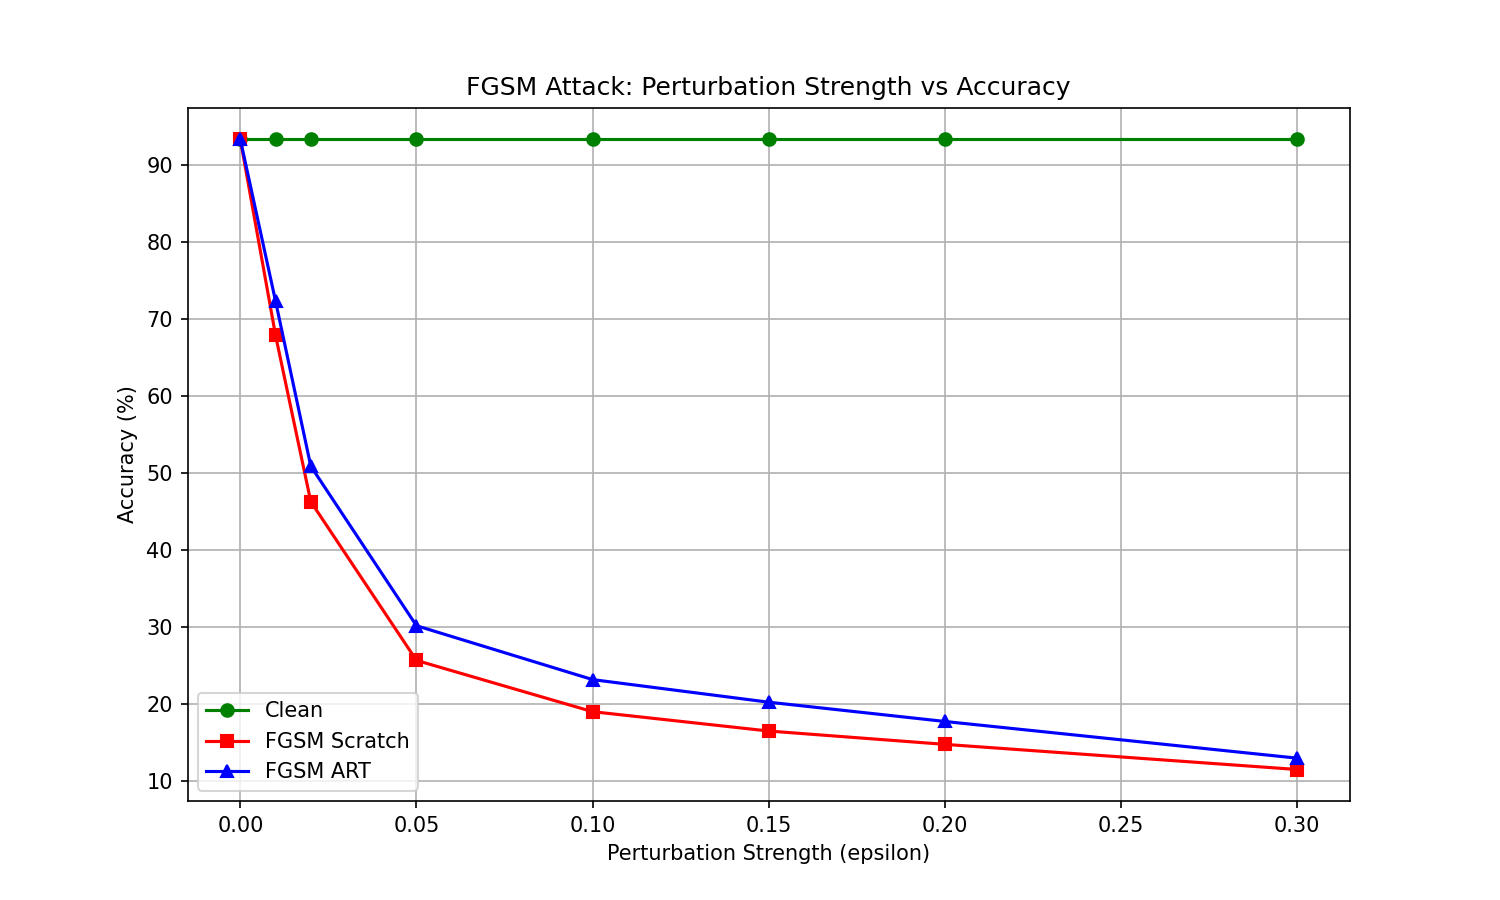
\includegraphics[width=0.72\textwidth]{figures/fgsm_eps_comparison.png}
\caption{Perturbation strength ($\epsilon$) vs model accuracy under FGSM attack. Both implementations cause catastrophic accuracy drops, with the scratch version being slightly more aggressive.}
\end{figure}

\subsubsection{Visual Comparison}

\begin{figure}[H]
\centering
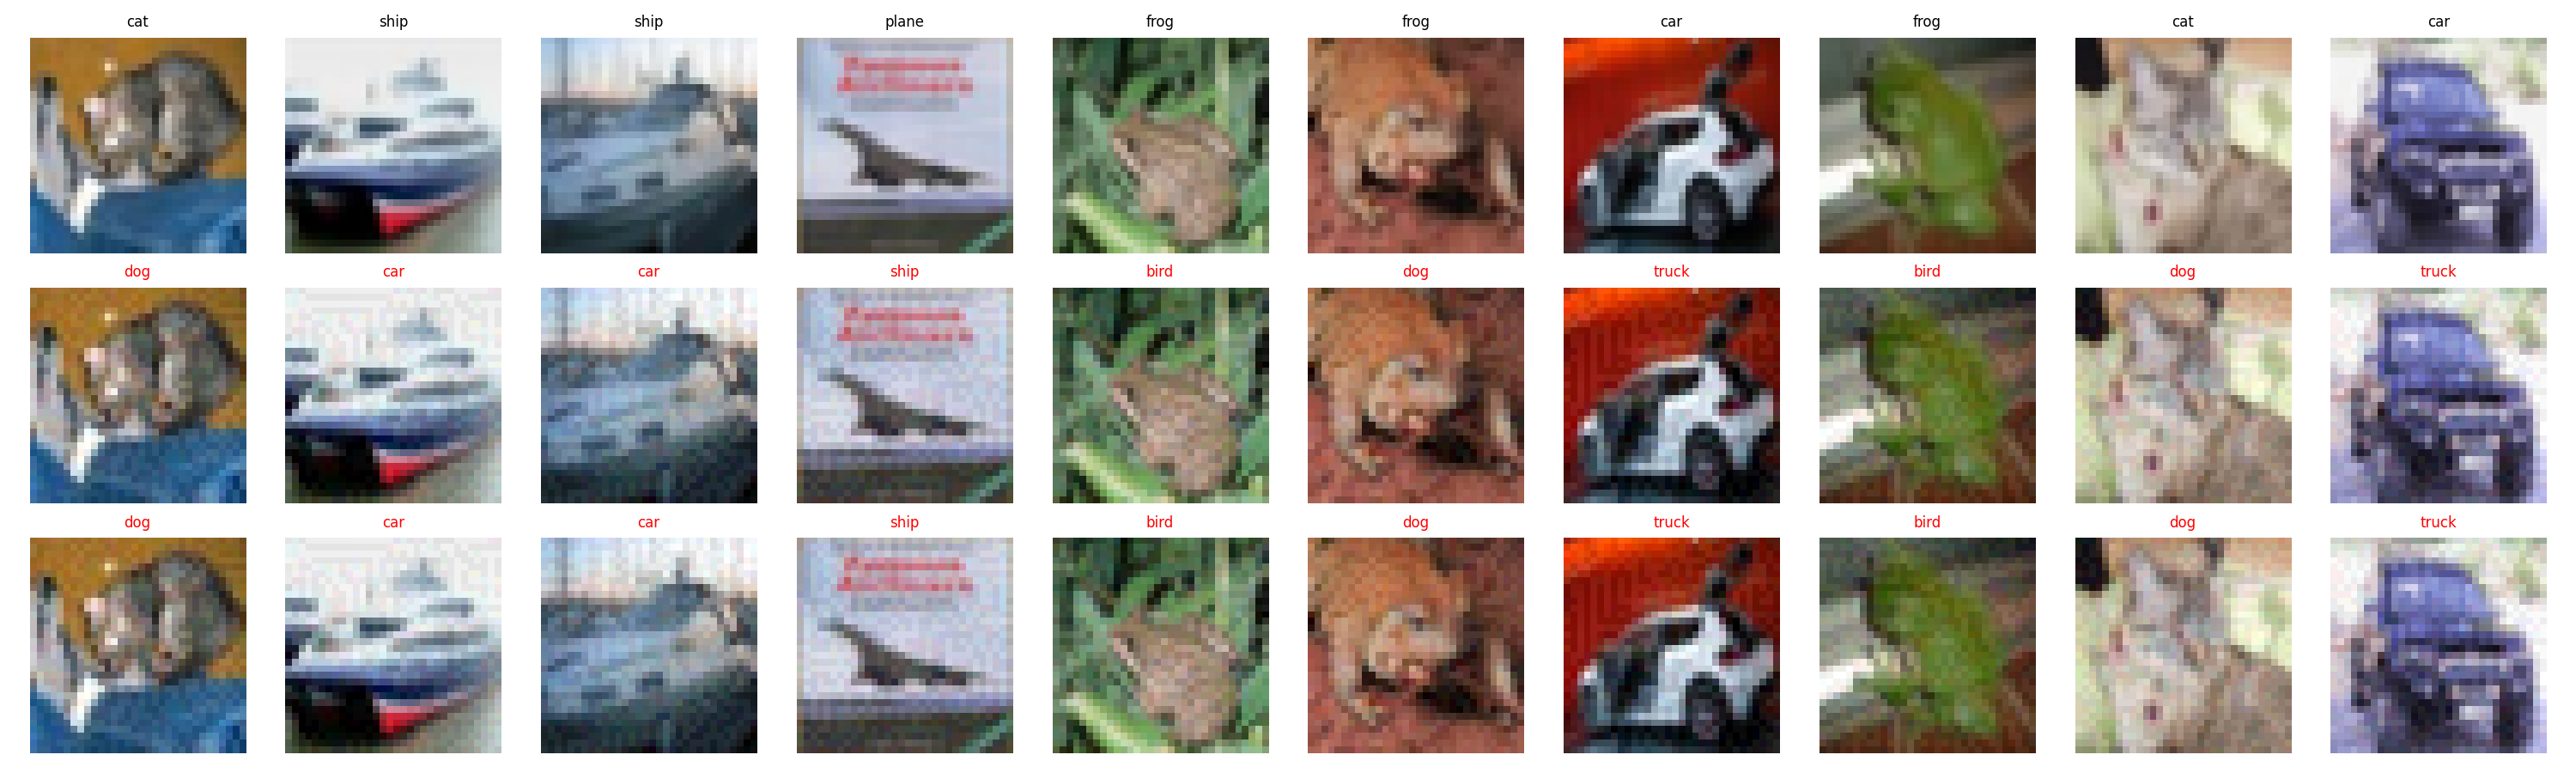
\includegraphics[width=0.95\textwidth]{figures/fgsm_visual_comparison.png}
\caption{Top: original images. Middle: FGSM from scratch ($\epsilon$\,=\,0.1). Bottom: FGSM via IBM ART ($\epsilon$\,=\,0.1). Red titles indicate misclassification.}
\end{figure}

\subsubsection{Analysis}

FGSM is remarkably effective: even at $\epsilon = 0.01$, accuracy drops from 93.35\% to 66--70\%.
At $\epsilon = 0.1$, accuracy plummets below 20\%, despite the perturbations being largely imperceptible to humans.

The ART implementation yields 2--5\% higher adversarial accuracy compared to the scratch version.
This difference arises because ART applies additional numerical safeguards such as gradient clipping and careful handling of floating-point precision, producing slightly less aggressive perturbations.

The key takeaway is that standard DNNs are highly vulnerable to even single-step gradient-based attacks, motivating the need for adversarial training or certified defenses.

%----------------------------------------------------------------------
\subsection{Q2(ii): Adversarial Detection Model}

\subsubsection{Setup}
ResNet-34 binary classifiers were trained to distinguish clean images from adversarial images.
Adversarial examples were generated using IBM ART's PGD and BIM attacks with $\epsilon = 0.15$, step size 0.02, and 20 iterations on 10,000 CIFAR-10 training images.
The detector was trained for 25 epochs with Adam (lr\,=\,0.001).

\subsubsection{Adversarial Sample Visualization}

\begin{figure}[H]
\centering
\begin{subfigure}{0.48\textwidth}
    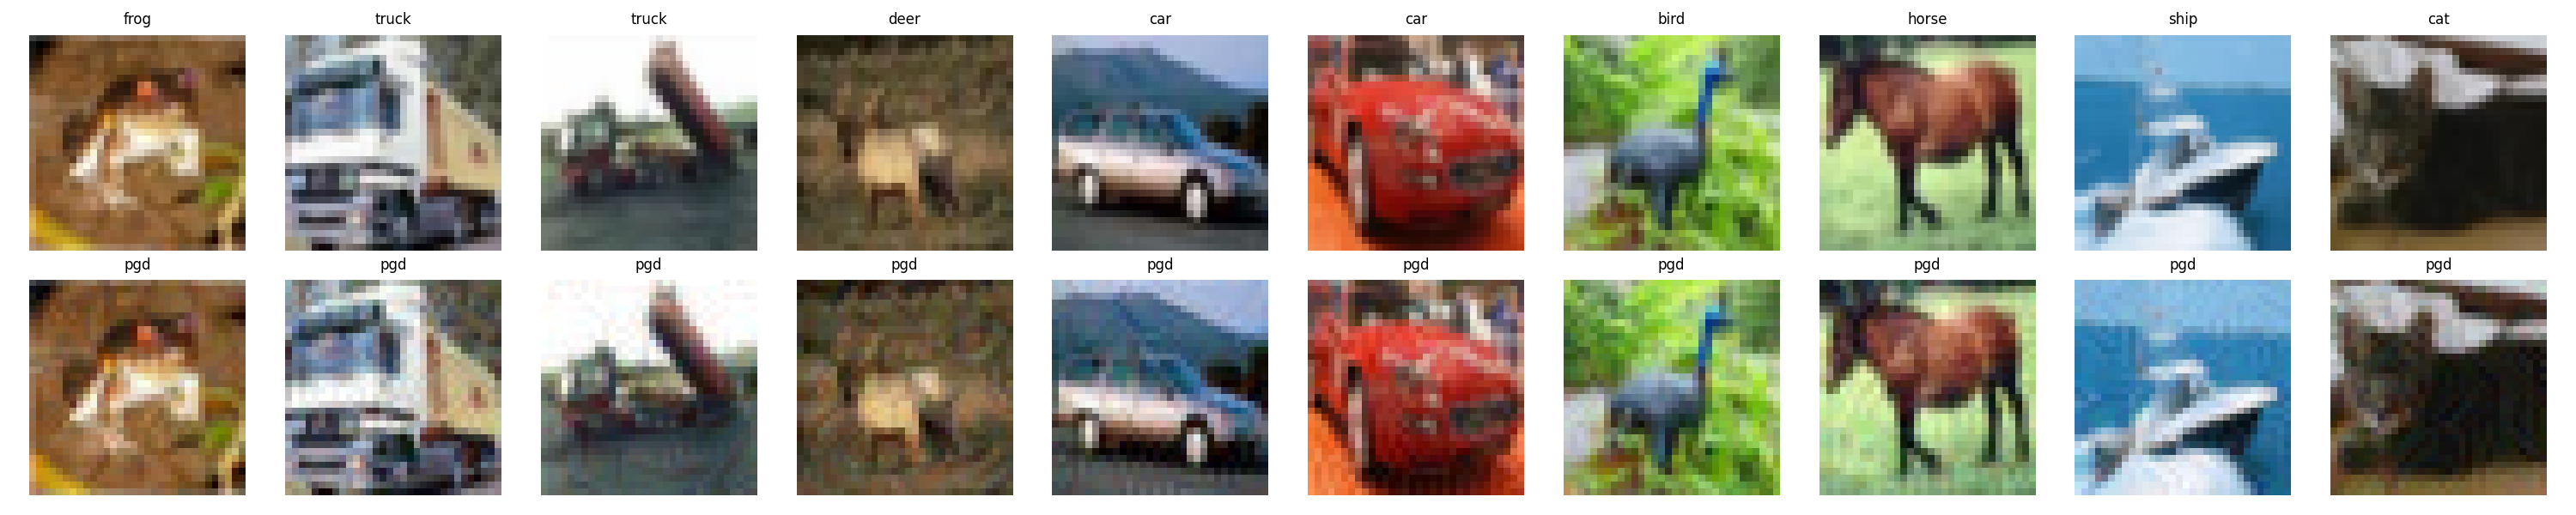
\includegraphics[width=\textwidth]{figures/samples_pgd.png}
    \caption{PGD attack samples}
\end{subfigure}
\begin{subfigure}{0.48\textwidth}
    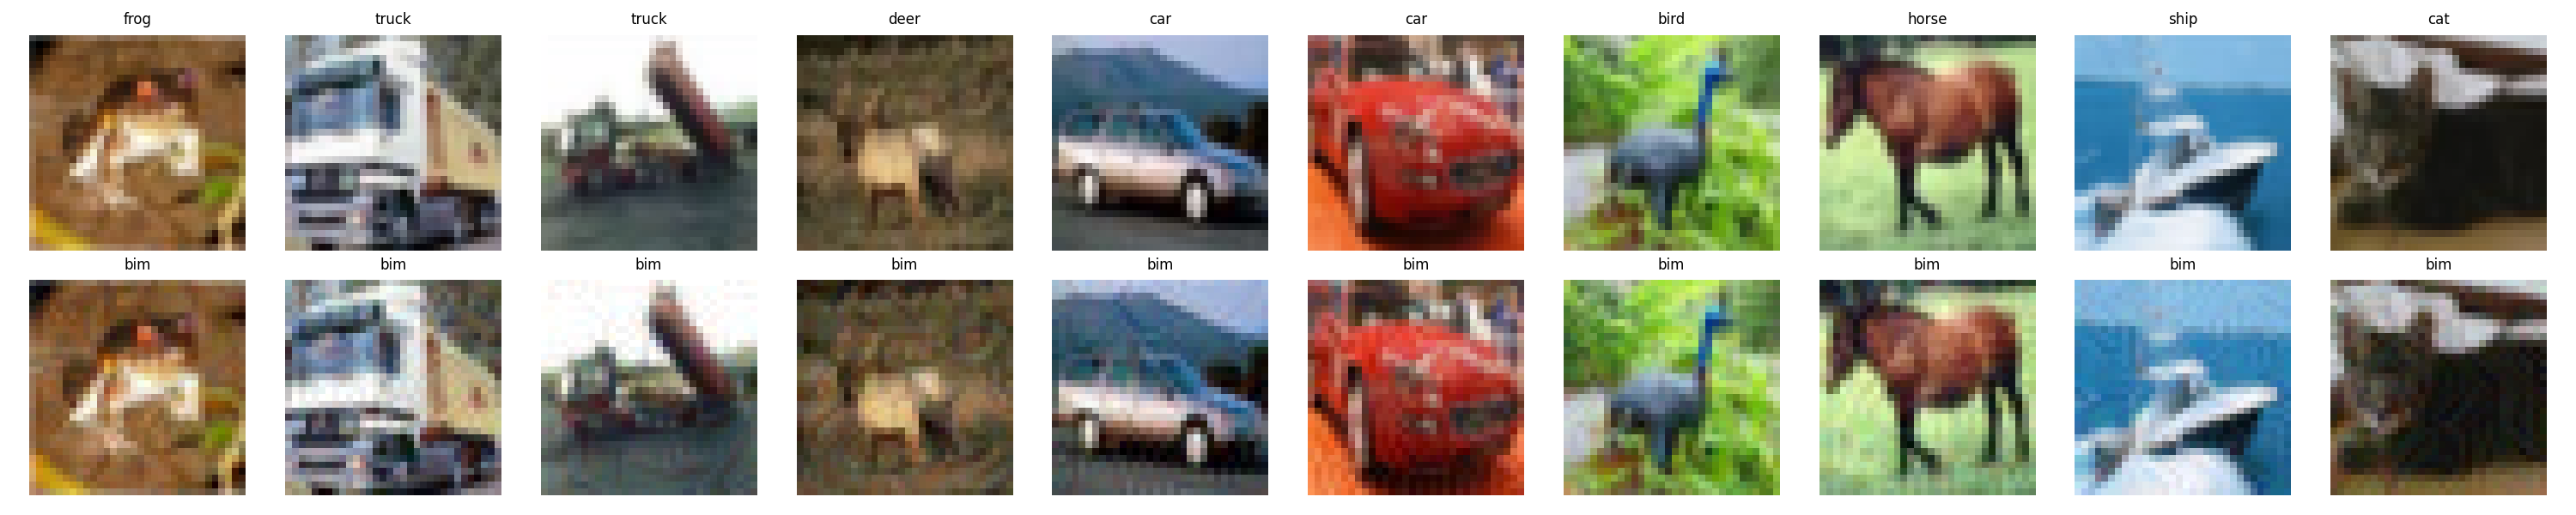
\includegraphics[width=\textwidth]{figures/samples_bim.png}
    \caption{BIM attack samples}
\end{subfigure}
\caption{Clean (top row) vs adversarial (bottom row) images for PGD and BIM attacks ($\epsilon = 0.15$).}
\end{figure}

\subsubsection{Detection Results}

\begin{table}[H]
\centering
\caption{Adversarial Detection Accuracy (binary: clean vs adversarial)}
\begin{tabular}{lc}
\toprule
Attack Type & Detection Accuracy (\%) \\
\midrule
PGD (Projected Gradient Descent) & \textbf{99.15} \\
BIM (Basic Iterative Method) & \textbf{99.90} \\
\bottomrule
\end{tabular}
\end{table}

Both detectors achieve $\gg 70\%$ detection accuracy.

\subsubsection{Analysis}

PGD and BIM are both iterative extensions of FGSM.
PGD applies FGSM repeatedly with random initialization and projects perturbations back onto the $\epsilon$-ball after each step.
BIM applies FGSM iteratively with small step sizes without random restarts.

With $\epsilon = 0.15$ and 20 iterations, both attacks produce perturbations that introduce detectable statistical artifacts.
The ResNet-34 detector learns to identify subtle patterns in the spatial and frequency domains of adversarial images that deviate from natural image statistics.

BIM achieves slightly higher detectability (99.90\% vs 99.15\%) because its perturbations follow a more uniform, predictable pattern without random restarts, making them marginally easier to distinguish from clean data.

The near-perfect detection rates demonstrate that adversarial perturbations, while imperceptible to humans, leave identifiable statistical fingerprints that deep learning models can exploit for detection.

Full sample visualizations (10 clean + adversarial pairs for FGSM, PGD, and BIM) are available on WandB:
\url{https://wandb.ai/b22cs093-prom-iit-rajasthan/adversarial-cifar10}

%======================================================================
\section{Conclusion}
%======================================================================

\begin{enumerate}
    \item \textbf{LoRA for ViT:} LoRA enables parameter-efficient fine-tuning of ViT-S on CIFAR-100. The best configuration (R\,=\,8, $\alpha$\,=\,8) achieves 85.40\% test accuracy using only 0.68\% of the model's parameters, surpassing the head-only baseline by 4.29\%.

    \item \textbf{Rank and Alpha:} Both rank and alpha have a strong positive effect on accuracy. Higher rank increases the expressivity of the low-rank adaptation, while higher alpha amplifies the learned update signal. Optuna confirmed R\,=\,8, $\alpha$\,=\,8 as optimal with a tuned LR of 0.00564.

    \item \textbf{FGSM Vulnerability:} A single gradient step (FGSM) can reduce a 93\% accurate model to below 20\% at $\epsilon = 0.1$. Both scratch and ART implementations produce similar results, with ART being marginally less aggressive due to numerical safeguards.

    \item \textbf{Adversarial Detection:} Deep learning-based detectors (ResNet-34) achieve near-perfect accuracy (99.15\% PGD, 99.90\% BIM) in distinguishing clean from adversarial images, demonstrating that adversarial perturbations leave detectable statistical fingerprints despite being imperceptible to humans.
\end{enumerate}

\end{document}
